% !Mode:: "TeX:UTF-8"
% !TEX root = ..\Literature_Translation.tex
\kchapter{建立解决方法}
本章我们将建立该问题的解决方法。首先,我们先将引入作业划分概念,并结合批量作业以减少换线时间、提高装配车间效率。而后,我们建立两个最优化特点,并提出了一个整数规划(MIP)公式以导出最优解。最后,我们提出了三个启发式方法以得到近似最优解。
\ksection{作业划分和批量作业}
为了改善现行的调度方法,我们引入了多批次发货(Bukchin,2002)概念,并打算用作业划分策略将作业划分成几个子作业。将作业划分策略结合入批量处理后,$c$项子作业便可分开同时由$c$个工人来处理。这样一来,可以避免相互干涉,减少等待时间。由于这些子作业都在批量中心,并且是连续离开机器,这$c$位工人必须同时停止作业,否则一些工人可能会处于闲置状态,而另一些工人却还在忙。
可以运用模块化设计和标准化以确保这$c$位工人同时停止作业,这样一来所工作拥有同样的处理时间,$c$位工人可以的工作强度近似一致。
如有必要,这4位工人可以互相帮工,这样一来,这些子作业可以同时完成。
因此,处理可以变得更为流畅,并且在工段1不会产生瓶颈。如\reff{fig:bwf}所示,接下来整个系统可以看作一个两阶段流水车间,工段1有4工人操作的批处理机器,工段2有2工人操作的离散机器。

承前所述,我们在工段1将作业划分成$c$项子作业,必须由$c$位工人同时操作,这样他们可以看作一个容量为$c$项作业的批量处理机器(Liu 和Yu,2000)。批$i$的处理时间为在此批中的最长作业处理时间,即$p_1(B_i)=\max p_{1j}=p_1$。
此外,每当一个新的批量产生,都需要考虑批量换线时间$s_b$,同样,开始首项作业或切换不同产品簇的作业时,需要考虑产品簇换线时间$s_{f1}$。
需要注意的是,批量中的最后一个作业或者同产品簇的下批首个作业不需要考虑产品簇换线时间。如此一来,批次$i$的完工时间$C_{1,[i]}$等于批量启动时间加上批量换线时间加上同批的产品簇换线和作业处理时间,即:
\begin{gather}
C_{1,[0]}=0 \label{equ:1} \\
C_{1,[i]}=C_{1,[i-1]} + s_b + s_{f1}\sum_{r=1}^c k_{1,[i,r]} + p_1 \label{equ:2}\\
(i=1,...,b, \text{如果}f_{1,[i,r]}=f_{1,[i,r-1]}\ k_{1,[i,r]}=0, \text{否则}k_{1,[i,r]}=1 )\notag
\end{gather}

作业在工段2用离散机器处理,作业按批进入但是一个接一个离开。开始首项工作或者切换产品簇的时候需要考虑产品簇换线时间$s_{j2}$。$J_{[j]}$的完工时间$C_{2,[j-1]}$等于$C_{1,[i]}$或者$C_{2,[j-1]}$加上$J_{[j]}$的产品簇换线时间和作业处理时间,即:
\begin{gather}
C_{2,[0]}=0\label{equ:3}\\
C_{2,[j]}=\max\{C_{1,[i]},C_{2,[j-1]}\} + s_{f2}\times k_{2,[j]} + p_{2,[j]}\label{equ:4}\\
(i=1,...,b,j=1,...,n \text{如果}f_{2,[j]}=f_{2,[j-1]}\ k_{2,[j]}=0, \text{否则}k_{2,[j]}=1)\notag 
\shortintertext{如此一来,}
C_{\max}=C_{2,[n]}\label{equ:5}\\
\sum_{j=1}^n T_j = \sum_{j=1}^n \max\{C_{2,[j]}-d_{[j]},0\}\label{equ:6}\\
Z = \alpha C_{\max} + \beta\sum_{j=1}^n C_{2,[j]} + \gamma\sum_{j=1}^n T_j  \label{equ:7}
\end{gather}

为了提高一次完成率,我们只接受滞后和小于$20\ h$每周的调度,因为滞后作业可以适当的周末里加班解决。否则,生产管理员需要和销售人员协商更改滞后作业的完工时间并重新调度。
\ksection{性质发掘}
\newcounter{prop}\newcounter{exam}
%\renewcommand{\theprop}{\arabic{prop}.}
\theoremheaderfont{\heiti}
\newtheorem{propetry}[prop]{性质}
\newtheorem{example}[exam]{例}

定义有$c$项作业的批为一个完整批,并称不足量的为局部批。回想一下,我们假设作业的数量为批量的倍数,即$n=b\times c$。

\begin{propetry}
对于案例问题来说,最优调度中的所有批皆为完整批。
\end{propetry}
\begin{proof}
记$S'$为一个包含一些完整批和局部批的序列,即$B_1,B_2,...,B'_k,B'_{k+1},...,B'_{b'}$。我们将第2个局部批$B'_{k+1}$的部分作业移到第1个局部批$B'_k$中,使之成为一个完整批$B_k$。重复这个步骤直到我们得到一个包含所有完整批($B_1,B_2,...,B_k,B_{k+1},...,B_b$)的序列$S$。这样一来,$S$中的作业开始时间要小于(对于$B'_k$之后的那些作业)等于(对于剩下的那些作业)$S'$,完工时间亦复如是。因此,就目标函数值来说,$S\text{主导了}S'$,证明完毕。
\end{proof}
\begin{propetry}
在最优调度中,同批中相同产品簇的作业必须连续处理。
\end{propetry}
\begin{proof}
读者可以参阅Baker(1999)和Chandru(1993)等的相关文献。
\end{proof}

在这两个性质的前提下,我们可以缩小MIP 模型和启发式方法的研究范围,以求得作业量为批量倍数的最优或近似最优调度,并将大大节省计算时间。
此外,我们采用$80/20$混合MTO/MTS 法则以应对紧急插单。
因此,当MTO 中的作业不足1批的时候,
生产管理员可以从MTS 中选取作业将其补足。

\ksection{~MIP 公式}
在MIP公式中的变量定义如下:
\begin{itemize}
\itemsep=0pt\parskip=0pt\parsep=0pt
\item 作业批次分派

$X_{j,[i,r]}$,0--1变量,在工段1如果$J_j$安排入批$i$的第$r$位置,那么取$1$,否则取$0$。
\item 簇换线时间

$k_{1,[i,r]}$,0--1变量,在工段1如果在批$i\text{第}r$位置的作业需要考虑簇换线时间,那么取$1\text{,否则取}0$。
\item 辅助变量

$g_{i,[r,]}$,0--1变量,用于产生$k_{1,[t,r]}$。
\end{itemize}

同时,完工时间和滞后时间皆为非负连续变量。这样一来,由\eqref{equ:1} -- (\ref{equ:7})即上述的两个性质,案例问题可以描述成如下MIP 模型:
\begin{gather}
\text{Minimize}\qquad \alpha C_{\max}+\beta\sum_{j=1}^n C_{2,[j]}+\gamma\sum_{j=1}^n T_j \label{equ:8}
\end{gather}
\begin{align}
&\text{s.t.}\notag\\
& \sum_{j=1}^n\sum_{r=1}^c X_{j,[i,r]} = c,\quad i=1,...,b\label{equ:9}\\
& \sum_{i=1}^b\sum_{r=1}^c X_{j,[i,r]} = 1,\quad j=1,...,n\label{equ:10}\\
& \sum_{j=1}^n X_{j,[i,r]} = 1,\quad i=1,...,b, r=1,...,c\label{equ:11}\\
&f_{1,[i,r]} = \sum_{j=1}^n X_{j,[i,r]}f_j,\quad i=1,...,b, r=1,...,c\label{equ:12}\\
&f_{2,[(i-1)\times c + r]} = \sum_{j=1}^n X_{j,[i,r]}f_j,\quad i=1,...,b, r=1,...,c\label{equ:13}\\
&d_{[(i-1)\times c + r]} = \sum_{j=1}^n X_{j,[i,r]}f_j,\quad i=1,...,b, r=1,...,c\label{equ:14}\\
&p_{2,[(i-1)\times c + r]} = \sum_{j=1}^n X_{j,[i,r]}p_{2j}\label{equ:15}\\
&k_{1,[1,1]} = 1\label{equ:16}\\
&f_{1,[i,r]}-f_{1,[i,r-1]} = - 3g_{i,[r,1]} - 2g_{i,[r,2]} - g_{i,[r,3]} + g_{i,[r,5]} + 2g_{i,[r,6]} + 3g_{i,[r,7]},\quad i=1,...,b, r=2,...,c\label{equ:17}\\
&g_{i,[r,1]} + g_{i,[r,2]} + g_{i,[r,3]} + g_{i,[r,4]} + g_{i,[r,5]} + g_{i,[r,6]} + g_{i,[r,7]} = 1,\quad i=1,...b, r=2,...,c\label{equ:18}\\
&k_{1,[i,r]} = g_{i,[r,1]} + g_{i,[r,2]} + g_{i,[r,3]} + g_{i,[r,5]} + g_{i,[r,6]} + g_{i,[r,7]},\quad i=1,...b, r=2,...,c\label{equ:19}\\
&f_{1,[i,1]}-f_{1,[i-1,c]} = - 3g_{i,[1,1]} - 2g_{i,[1,2]} - g_{i,[1,3]} + g_{i,[1,5]} + 2g_{i,[1,6]} + 3g_{i,[1,7]},\quad i=2,...,b\label{equ:20}\\
&g_{i,[1,1]} + g_{i,[1,2]} + g_{i,[1,3]} + g_{i,[1,4]} + g_{i,[1,5]} + g_{i,[1,6]} + g_{i,[1,7]} = 1,\quad i=2,...b\label{equ:21}\\
&k_{1,[i,1]} = g_{i,[1,1]} + g_{i,[1,2]} + g_{i,[1,3]} + g_{i,[1,5]} + g_{i,[1,6]} + g_{i,[1,7]},\quad i=2,...b\label{equ:22}\\
&k_{2,[(i-1)\times c + r]} = k_{1,[i,r]},\quad i=1,...,b, r=1,...,c\label{equ:23}\\
&C_{1,[0]} = 0\label{equ:24}\\
&C_{1,[i]} = C_{1,[i-1]} + s_b + s_{f1}\sum_{r=1}^c k_{1,[i,r]} + p_1,\quad i=1,...,b\label{equ:25}\\
&C_{2,[0]} = 0\label{equ:26}\\
&C_{2,[(i-1)\times c + r]} = \max \{C_{1,[i]},C_{2,[(i-1)\times c + r]}\} + s_{f2}k_{2,[(i-1)\times c + r]} + p_{2,[(i-1)\times c + r]},\quad i=1,...b-1, r=1,...,c\label{equ:27}\\
&C_{\max} = C_{2,[n]}\label{equ:28}\\
&T_j = \max\{C_{2,[j]}-d_{[j]},0\},\quad j=1,...,n\label{equ:29}\\
&X_{j,[i,r]},k_{1,[i,r]},k_{2,[j]} = 0 \text{或} 1,\quad j=1,...,n, i=1,...,b, r=2,...,c\label{equ:30}\\
&g_{i[r,l]} = 0 \text{或} 1,\quad i=1,...,b, r=2,...,c, l=1,...,7\label{equ:31}
\end{align}

考虑到\eqref{equ:27}和\eqref{equ:29}是非线性的,但他们可以较为容易的转化为线性形式。例如,约束条件(\ref{equ:27})可以改写为
\begin{numcases}{}
C_{2,[(i-1)\times c + r]}\geqslant C_{1,[i]} + s_{f2}k_{2,[(i-1)\times c + r]} + p_{2,[(i-1)\times c + r]} \notag\\
C_{2,[(i-1)\times c + r]}\geqslant C_{2,[(i-1)\times c + r - 1]} + s_{f2}k_{2,[(i-1)\times c + r]} + p_{2,[(i-1)\times c + r]}\notag
\end{numcases}

我们现在来解释一下这个MIP 公式。目标函数(\ref{equ:8})是最小化加权制造期和、完工时间和、总滞后时间和三者之和。约束条件(\ref{equ:9})确保每一批次正好有$c$项作业,约束(\ref{equ:10})和(\ref{equ:11})确保作业和批次的位置一一对应。\eqref{equ:12}确定了工段1中批$i$第$r$位置的作业簇,约束(\ref{equ:13}) -- (\ref{equ:15})确定了安排在工段2的作业产品簇、工期和处理时间,\eqref{equ:16} -- (\ref{equ:22})确定了$k_{1,[i,r]}$。
由于\eqref{equ:17}左边为非0--1变量,即$f_{1,[i,r]}-f_{1,[i,r-1]}=\{-3,-2,-1,0,1,2,3\}$,需要增加辅助变量$g_{i,[r,l]}$和约束(\ref{equ:17}) -- (\ref{equ:22})以确保该模型为一个MIP 问题(Hillier 和Liberman,2001)。
如果在工段1作业$[i,r]$和其前继作业属于同一簇,那么$k_{1,[i,r]}=0\text{,否则}k_{1,[i,r]}=1$。约束条件(\ref{equ:23})产品簇换线变量$k_{2,[j]}$。
由于所有作业流程在系统中的顺序一致,所以$k_{2,[j]}=k_{1,[i,r]}$。\eqref{equ:24}和(\ref{equ:25})确定了工段1的完工时间,\eqref{equ:26}和(\ref{equ:27})确定了工段2的完工时间,并确保作业只有在其前继作业和本身完成了工段1的处理后才能开始操作。\eqref{equ:28}和(\ref{equ:29})确定了案例问题的运行情况度量,\eqref{equ:30}和(\ref{equ:31})是0--1变量约束。

\begin{example}
作为一个例证,考虑一个有12项工作的问题,$f_j=(3,2,3,4,1,4,2,2,3,3,4,4),d_j=(100,160,160,100,180,\\
140,140,140,140,140,180,140),s_b=6.4,s_{f1}=3.2,s_{f2}=1.6$,其他数据见\reft{tab:2yearproduction}。\label{exam:1}
\end{example}

可以用LINGO 10 来解决这个MIP 问题,我们可以得到最优结果如下:

在$(\alpha,\beta,\gamma) = (0.6,0.2,0.2)$下的目标函数值为
$$Z = 331.04, C_{\max} = 164.0, {\textstyle\sum_j C_j = 1163.2}, T_{\max} = 0$$

各指派值为
\begin{align*}
 X_{10,[1,1]} & = 1 & X_{3,[1,2]} & = 1 & X_{1,[1,3]} & = 1 & X_{9,[1,4]} & = 1\\
 X_{4,[2,1]} & = 1 & X_{11,[2,2]} & = 1 & X_{12,[2,3]} & = 1 & X_{6,[2,4]} & = 1\\
 X_{8,[3,1]} & = 1 & X_{7,[3,2]} & = 1 & X_{2,[3,3]} & = 1 & X_{5,[3,4]} & = 1
\end{align*}

所有其他的指派值为0。

产品簇换线变量为
\begin{align*}
k_{1,[1,1]} & = 1 & k_{1,[2,1]} & = 1 & k_{1,[3,1]} & = 1 & k_{1,[3,4]} & = 1 \\
k_{2,[1]} & = 1 & k_{2,[5]} & = 1 & k_{2,[9]} & = 1 & k_{2,[12]} & = 1
\end{align*}

所有其他的产品簇换线变量皆为0。最优调度的Gantt 图如\reff{fig:gantt1}所示。
\begin{figure}[h]
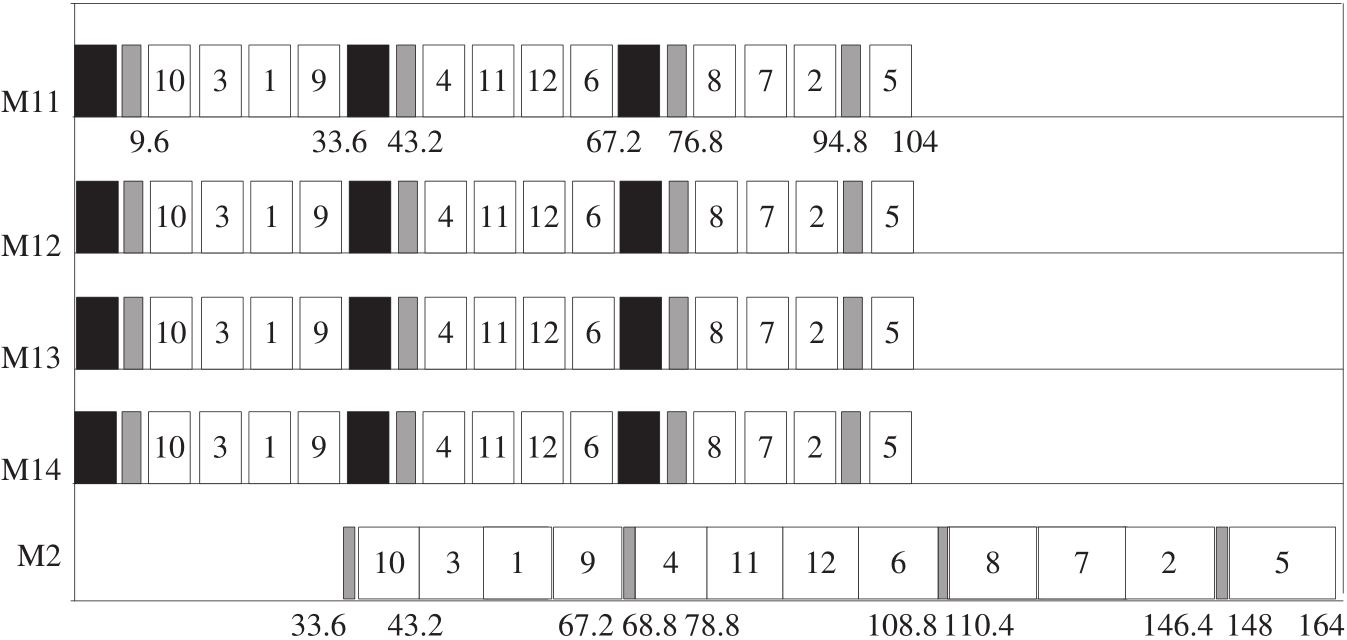
\includegraphics[width=10cm]{ganttexam1.jpg}
\caption{例\ref{exam:1}最优调度的Gantt 图\label{fig:gantt1}}
\end{figure}

这个MIP 公式可以用来求解只有少量的作业和产品簇,对于通常问题的调度求解十分困难。实际情况中,我们可能遇到大量作业和产品簇的问题,所以建立启发式方法变得十分重要,这些方法可以较快解决中、大型问题的近似最优解。

\ksection{启发式方法}
在2.5节中,我们解释了现行的单件处理和EDD 规则调度方法。为了有效解决涌现的问题和提高调度效果,我们提出了启发式方法。
\newcommand{\Step}{{\heiti 步骤}}

\ksubsection{启发式方法1:FBEDD}
我们将EDD 规则结合完整批的性质,建立了一个完整批EDD (FBEDD)启发式方法,以最小化目标值,具体步骤如下

\begin{asparaenum}
\renewcommand{\labelenumi}{\heiti 步骤\theenumi~}
\item 置$S=\phi,\ S_U = \{J_1,J_2,...,J_n\},\ B=\phi,\ i=1,2,...,b,\ b = n/c$。
\item 将$S_U$中的作业按$d_j$非减的顺序排列,置$i=1$。
\item 将$S_U$中的前$c$项作业组成批次$B_i$,即$B_i = \{J_{[1]},...,J_{[c]}\}$。
\item 如果$S_U = \phi$,则执行\Step5,否则$i=i+1$,并执行\Step 3。
\item 最终的调度为$S=B=(B_1,...,B_b)$。
\end{asparaenum}

\ksubsection{启发式方法2:FBFS}
作业要群组成一些产品簇的集合。我们选用同簇中的$c$项作业组成一个完整批,然后把不同簇中剩余的作业组成最后一批,这批的作业按最短处理时间(SPT)规则排序。这个启发式方法的步骤叫做完整批簇排序(FBFS)启发式算法,如下所示。其中$\# F^f$表示产品簇作业$f$的集合$F^f$的作业数量。
\begin{asparaenum}
\renewcommand{\labelenumi}{\heiti 步骤\theenumi~}
\item 置$S_1 = \phi,\ S_2=\phi,\ S_U = \{J_1,...,J_n\},\ B = \phi,\ B' = \phi,\ b=n/c$。
\item 将$S_U$中的作业按$d_j$非减的顺序排列。
\item 将得到的序列作业按产品簇排序以组成集合,置$f=1$。
\item 如果$\# F^f \geqslant c$,执行\Step 7,否则执行\Step 5。
\item 置$i=1$,将$F^f\text{并入}B'_i$作为一个局部批,然后从$S_U\text{剔除}B'_i$。
\item 如果$S_U = \phi$,执行\Step 9,否则置$f=f+1$,并执行\Step 4。
\item 置$i=1$,从$F^f$中拿出前$c$项作业作为一个完整批$B^f_i$,将至并入$B$,并从$S_U\text{中剔除}B^f_i$。
\item 如果$\# F^f \geqslant c$,执行\Step 7,否则执行\Step 5。
\item 置$B = \{B_1^1,...,B_i^1,...,B_1^4,...,B_i^4\},\ B' = \{B'_1,...,B'_4\}$。按$p_{2j}$非减的顺序排列重排$B'$中的作业。
\item 在作业顺序不变的情况下,重新定$B\text{与}B'$中的指数。置$B=\{B_1,...,B_{k-1}\}\text{并且}B' = \{B_k,B_{k+1},...,B_b\}$均为完整批。
\item 最终调度为$S=B\cup B' = \{B_1,B_2,..,B_b\} = \{J_{[1]},J_{[2]},...,J_{[n]}\}$。
\end{asparaenum}

我们来解释以上的步骤。在\Step1和\Step2中,我们构建了一个初始调度,作业是按EDD 规则排序的。在\Step3中,作业群组成4个簇。\Step4 -- 8,我们取各簇前$c$项作业组成一个完整批,并将剩余的作业组成一个最后批。在\Step9,我们按SPT 规则重排了局部批的作业,以改良目标函数值。\Step10我们在不改变作业顺序的情况下,重新设置了各完整批的指数,以保证其完整。在\Step11,我们得到了最终调度方案。
\begin{example}
考虑一个12个作业的问题,其中$p_{aj}=9,s_a=5.2,p_{1j}=24,s_b=6.4,s_{f1}=3.2,s_{f2}=1.6$。其他数据同例\ref{exam:1}。
\end{example}
\begin{asparaenum}
\renewcommand{\labelenumi}{解\theenumi:}
\item 用EDD 规则求解该问题,得到最终调度:$C_{\max}=211,\ \sum C_j = 1419.0,\ \sum T_j = 66.2,\ Z(S)=408.32$。
\item 用FBEDD 规则求解该问题,得到最终调度:$C_{\max}=178.4,\ \sum C_j = 1344.4,\ \sum T_j = 0,\ Z(S)=375.92$。
\item 用FBFS 规则求解该问题,得到最终调度:$C_{\max}=164,\ \sum C_j = 1163.2,\ \sum T_j = 0,\ Z(S)=331.04$。
\end{asparaenum}
\ksubsection{启发式方法3:RFBFS}
当我们运用FBFS 求解大型问题的时候,换线时间和可以被最小化,然而,这个方法给出了同簇产品的优先级,却不顾工期。因此,这可能会耗费许多时间处理同簇产品的批次,导致一些作业被提前完成,而一些作业却要滞后完成。为了改善FBFS 的这个不足,我们融入了滚动时域调度策略以达成滚动完整批产品簇调度(RFBFS)的启发式方法。RFBFS 将大型问题分割成多个EDD 序列的小型问题,然后重复执行FBFS 直到所有作业都被调度。
由于RFBFS 运行FBFS 处理小型短时域问题,这样可以用于处理大型问题。该启发式方法的步骤如下,其中$n_b$表示每月可处理的批数。
\begin{asparaenum}
\renewcommand{\labelenumi}{\heiti 步骤\theenumi~}
\item 置$S_1 = \phi,\ S_U = \{J_1,...,J_n\},\ B_1 = \phi,\ B'_1 = \phi,\  n = b \times c$。
\item 将$S_U$中的作业按$d_j$非减的顺序排列,并置$\nu = 1$。
\item 从$S_U$中拿出前$n_b/2$项作业来执行FBFS,并产生一个局部调度$S_1 = B_1 \cup B'_1$。然后,置$\nu = \nu + 1$,并把剩下的$n_b/2$项作业执行FBFS,产生下一个局部调度$S_2 = B_2 \cup B'_2$。
\item 如果$S_U=\phi$,执行\Step5,否则,置$\nu = \nu + 1$,执行\Step3。
\item 最终的调度为$S=S_1\cup S_2\cup...\cup S_{\nu}$。
\end{asparaenum}

\ksection{确定下界}
为了评价启发式方法得到结果的质量,本节将引出下界。由于这些都是多目标函数,所以下界包含3个部分:\begin{inparaenum}[(1)]
\item $C_{\max}\text{的下界}LB_1$;
\item $\sum C_j\text{的下界}LB_2$;
\item $\sum T_j\text{的下界}LB_3$。
\end{inparaenum}
\renewcommand{\labelenumi}{}
\begin{asparaenum}
\item $C_{\max}\text{的下界}(LB_1)$
\suspend{asparaenum}

Ahmadi(1992)提出了LPT-Johnson 法则以最小化处理多簇产品的离散批系统的制造期。根据这个法则,作业在工段2按处理时间排列为非增序列。
为了得到合理的下界,我们融入了Azizoglu 和Webster(2003)提出的获得下界进程。
我们考虑将批换线时间$s_b$和产品簇换线时间$s_{f1}$计入工段1的处理时间,放宽工段2产品簇换线时间。
这样一来,下界可以由制造期加最小工段2簇换线时间($f_n \times s_{f2}$)得到。
记$C_{2,[j]}$(LPT)为$H_{[j]}$在工段2的完工时间,$f_n$为所有作业簇的数量,即:
\begin{numcases}{}
C_{2,[1]}(LPT) = (s_b + s_{f1} + p_1) + p_{2,[1]}\notag\\
C_{2,[j]}(LPT) = C_{2,[j-1]} + p_{2,[j]},\quad j=2,...,n\notag\\
LB_1 = C_{2,[n]}(LPT) + f_ns_{f2}\notag
\end{numcases}
\resume{asparaenum}
\item $\sum C_j\text{的下界}(LB_2)$
\suspend{asparaenum}

Ahmadi(1992)同时也提出完整批最短处理时间(Full Batch-SPT)法则以最小化工段2无闲置的离散批系统完工时间和。
根据这个法则,作业在工段2按处理时间排列为非减序列。
记$C_{2,[j]}$(SPT)为作业在工段2的完工时间,这样一来下界可由完工时间和加上工段2最小簇换线时间得到。簇换线时间只有在首个作业和末尾作业$f_n-1$时才考虑,即:
\begin{numcases}{}
C_{2,[1]}(SPT) = s_b + s_{f1} + p_1 + p_{2,[1]}\notag\\
C_{2,[j]}(SPT) = C_{2,[j-1]} + p_{2,[j]},\quad j=2,...,(n-f_n+1)\notag\\
C_{2,[j]}(SPT) = C_{2,[j-1]} + s_{f2} + p_{2,[j]},\quad j=(n-f_n+2),...,n\notag\\
LB_2 = \sum_{j=1}^n C_{2,[j]}(SPT) + (n+\sum_{k=1}^{f_n}(f_n-k))s_{f2}\notag
\end{numcases}
\resume{asparaenum}
\item $\sum T_j\text{的下界}(LB_3)$
\end{asparaenum}

Baker 和Martin(1974)证明SPT序列最小化了当所有作业都滞后的单机器滞后时间和。在这个离散批系统中,批处理时间相同,这样考虑由此引起的滞后和时,这个系统可以考虑为单个机器。
记$C_{2,[j]}$(SPT)为完工时间,$d_{[j]}$为SPT 顺序下$J_{[j]}$的工期。
这样一来,滞后时间和的下界可以由放宽所有作业皆滞后的约束得到,即:
\begin{numcases}{}
T_j = \max \{C_{2,[j]}(SPT)-d_{[j]}(SPT),0\},\quad j=1,...,n \notag \\
LB_3 = \sum_{j=1}^n T_j\notag
\end{numcases}

将这3个独立的下界综合,可以得到该问题的下界:
\[ LB = \alpha LB_1 + \beta LB_2 + \gamma LB_3
\]

为了评价启发式算法求解的质量,我们用相对误差(RER)定义启发式方法和下界的差别:
\begin{equation}
RER = \left( \frac{Heuristic_i - LB}{LB}\right)\times 100\%
\end{equation}
其中$Heuristic_i$是各启发式方法的目标函数值。